\chapter{需求分析与概要设计}

\section{需求分析}
\label{sec:requirements-analysis}

本视频编辑系统的需求分析基于技术可行性研究,主要涵盖目标用户分析、功能性需求分析与非功能性需求分析。

\subsection{用户分析}

本系统的目标用户分析如表~\ref{tab:system-users}所示。一方面该系统面向对最新人工智能技术感兴趣的研究者及普通用户,
需要提供简洁易用的界面和友好的交互体验;另一方面该系统面向实验室研究者,为他们提供了解用户真实需求的渠道,
包括相关的数据统计和分析功能。


\begin{table}
    \centering
    \bicaption{目标用户分析}{System Users Analysis}
    \label{tab:system-users}
    \resizebox{\linewidth}{!}{
    \begin{tabular}{cl}
        \toprule
        目标用户   &  用户特征与期望       \\
        \midrule
        专业人工智能研究人员 & 对算法研究较深,希望方便地得到已有工作成果的编辑结果用于对比或研究\\
        对算法感兴趣的非从业者 & 缺乏项目部署的理论基础,但又期望了解到最新研究成果,尝试最新算法的效果 \\
        本实验室的研究人员 & 期望将实验室算法部署到实际应用中,方便实验室成员获取用户反馈与需求 \\
        \bottomrule
    \end{tabular}
    }
\end{table}

\subsection{功能性需求分析}

在功能性需求方面,首先,多模态视频编辑功能应支持文本指令驱动、参考图像风格迁移、虚拟换装和光照调整等多种编辑方式,
允许用户自定义上传视频与编辑提示。其次,考虑到编辑过程需要预处理以及多轮训练,
系统无法实时的生成结果,因此需要在结果生成后通知用户并允许用户查看。最后,作为实验室算法的展示平台,系统需要
允许管理员用户导出统计信息以供研究使用。

\subsection{非功能性需求分析}

本系统的研发初衷是希望利用先进算法为用户提供方便快捷的编辑体验,同时作为实验室的展示平台与反馈信息来源,因此需要
在用户体验、数据安全、可维护性上满足用户需求。

\subsubsection{用户体验}

系统需要提供简洁易用的界面,包括友好的交互体验、合理的布局、外观的协调等,以方便用户快速上手。需要
避免过多的弹窗、信息等,以免干扰用户操作;同时,也需要在必要的时候提供提示与帮助信息,以帮助用户更好地使用系统。

\subsubsection{数据安全}

系统需要具备较高的安全性,应当采取的措施包括用户认证、数据库信息加密、前后端分离、
API接口鉴权等。另外由于系统部署在学校内网无法直接通过外网访问,需要网络地址转换(NAT)技术提供访问支持,
应当确保地址转换中网关能有效地阻止外部攻击。

\subsubsection{可维护性}
此外,系统应该具有较好的可维护性,包括代码规范、模块化设计、应用文档编写等,以方便后续的维护和升级。

\section{概要设计}

系统概要设计的主要任务是将一个复杂的系统按功能划分成模块,确定每个模块的功能及模块之间的调用关系;确定模块之间的
接口,即模块之间的数据传递方式。另外,根据系统涉及到的实体与实体间的关系,设计数据库的表结构。

\subsection{架构设计}

根据第一节所述的需求分析,我们采用分层微服务架构,结合事件驱动的设计模式,将系统划分为客户端层、服务层、数据层,如~\ref{fig:system-structure}所示。

客户端层通过组件管理、页面渲染提供响应式用户界面,并通过对服务层微服务的api调用处理用户交互事件;

服务层由Flask微服务集群组成,负责处理客户端请求,并与数据层通信进行数据存储和检索。服务层具体包括用户服务提供用户的注册、登录、找回密码等服务;
管理员服务提供数据统计与导出服务;编辑服务提供文件的上传、任务的上传与查询、任务的分发等服务。

数据层使用MySQL数据库存储用户信息、任务信息和编辑结果,使用Redis数据库存储任务队列和任务状态。

\begin{figure}[ht]
    \centering
    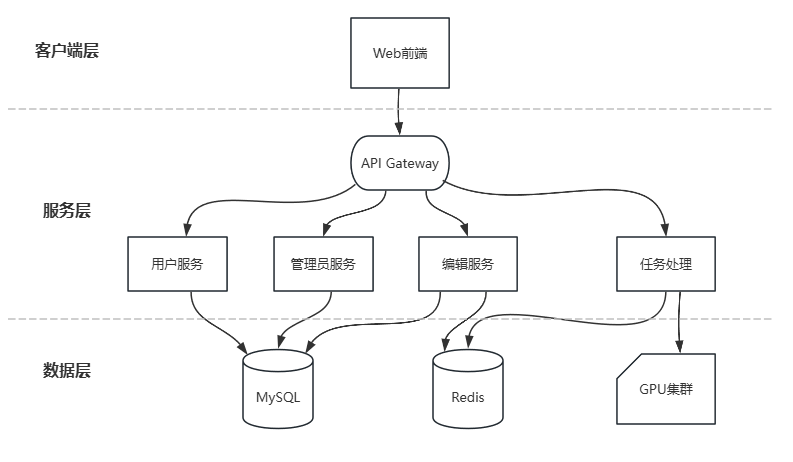
\includegraphics[width=0.5\textwidth]{source/img/system_structure.png}
    \bicaption{系统架构图}{System Architecture Diagram}
    \label{fig:system-structure}
\end{figure}

\subsection{4+1概要视图}

“4+1”视图是由Philippe Kruchten在1995年提出的一种软件架构描述方法。它将软件架构划分为四个视图,
包括逻辑视图、开发视图、物理视图和过程视图,以及一个场景视图。每个视图关注系统的不同方面,通过提供特定的抽象层次,
能够全面地描述系统的架构。场景视图关注系统的使用场景和用户需求,描述系统在特定场景下的行为和响应,我们已经在第一节
中详细地讨论过,下面我们着重通过其它四个视图来描述系统的架构设计。

\subsubsection{逻辑视图}

我们用用户用例图与逻辑流程来表示系统的逻辑设计,考虑到叙述方便,我们将在下一章具体实现系统时详细介绍这部分内容。

\subsubsection{开发视图}

考虑到我们使用的技术栈,Next.js直接通过文件结构定义api,因此我们的文件结构相对简单,只需要根据系统的具体路由来建立。
我们的大部分前端逻辑集中在pages下,components中存放了可复用的组件,包括自定义弹窗、自定义Hook等。在public中存放页面
使用到的静态资源,包括图片、图标等。前端使用的配置文件conf存放在attribute下,同时也包括css的样式文件。

后端被分为Flask API和Editor两个部分,考虑到我们的分层微服务架构,我们将Flask server分为Routes、Services、Utils三个部分。
Routes部分作为前端请求的入口,定义了后端路由并调用微服务;Services部分作为业务逻辑处理部分,具体实现了相应的微服务;Utils部分作为辅助工具,提供一些通用功能。

\begin{figure}[ht]
    \centering
    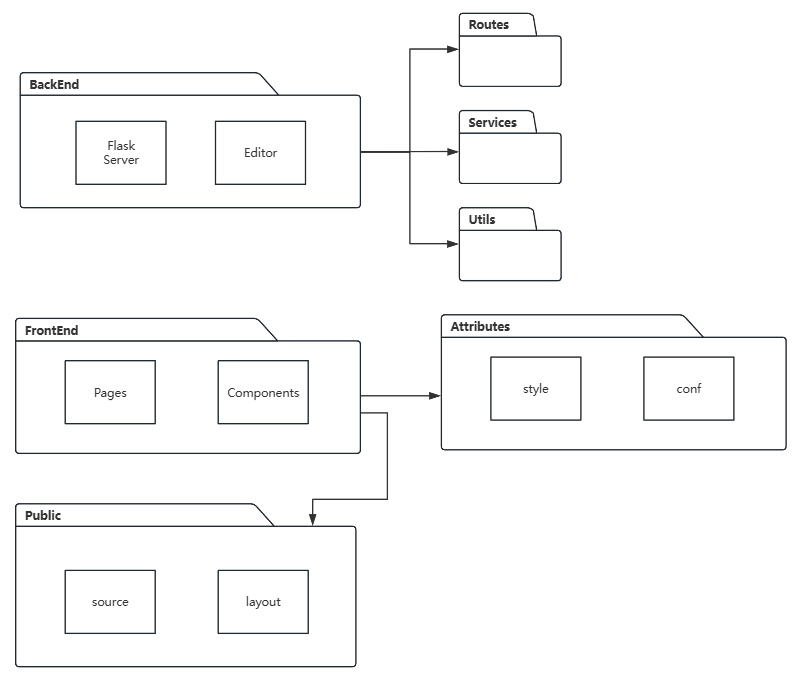
\includegraphics[width=0.6\textwidth]{source/img/system_develop.png}
    \bicaption{系统开发视图}{Development View}
    \label{fig:system-develop}
\end{figure}

\subsubsection{进程视图}

系统的进程视图从动态事件的角度描述系统的行为,包括系统对用户行为的相应、前端服务器对后端服务的调用、API调用等。我们
设计了如~\ref{fig:system-process}的进程视图,使用UML时序图来表示。

在我们的设计中,进程之间相互独立,互不影响。主要工作流为用户的任务请求上传与后端任务处理,后端接收到前端请求后将任务加入任务列表
等待分配给Worker,成功加入队列后就返回成功信息;而具体的任务处理则由Worker完成,不再返回前端,直到前端发起查询时通过数据库记录返回。
利用前端的条件判断,我们可以在一些情况下缩短进程,例如用户查询处理结果时,通过前端非“已完成”状态可以直接拦截请求,避免后端处理。

\begin{figure}[ht]
    \centering
    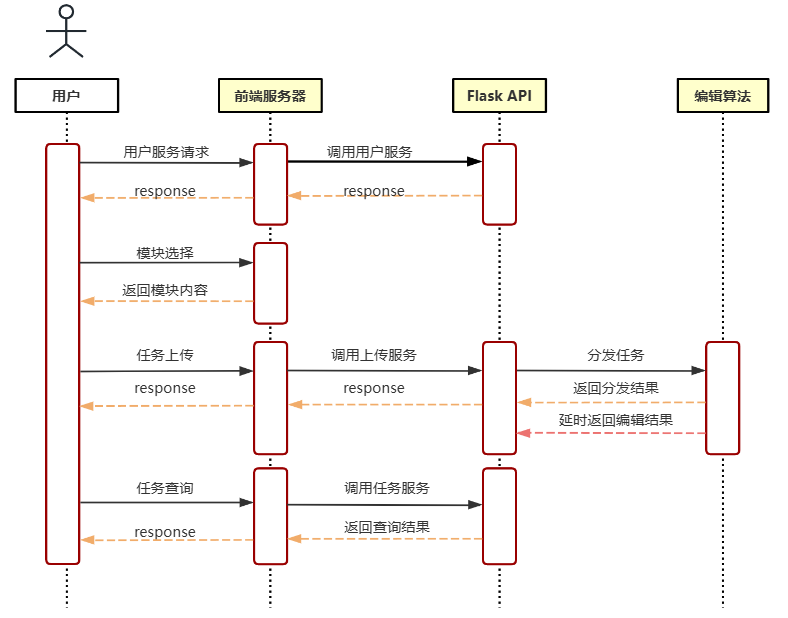
\includegraphics[width=0.7\textwidth]{source/img/system_process.png}
    \bicaption{系统进程视图}{Process View}
    \label{fig:system-process}
\end{figure}

\subsubsection{物理视图}

物理视图是从系统物理层面上部署架构的视角来整体描述系统结构的视图,我们设计的物理视图如~\ref{fig:system-deploy}所示。

预先渲染好的静态资源被部署在内容分发网络上(CDN)以加快用户的首屏加载,同时CDN通过负载均衡等技术使内容传输更快速、更稳定。
用户在浏览器通过HTTP协议向服务器发送请求,经过网关的网络地址转换发送到前端Next.js驻守的端口。前端服务器接收到网关分发
的请求后做出对应相应,并向后端Flask API驻守的端口跨域发送请求。Flask API调用相应的微服务并利用数据库操作完成响应,
同时后端初始时实例化Edit Work以接收Redis管理的任务队列,完成任务处理。

\begin{figure}[ht]
    \centering
    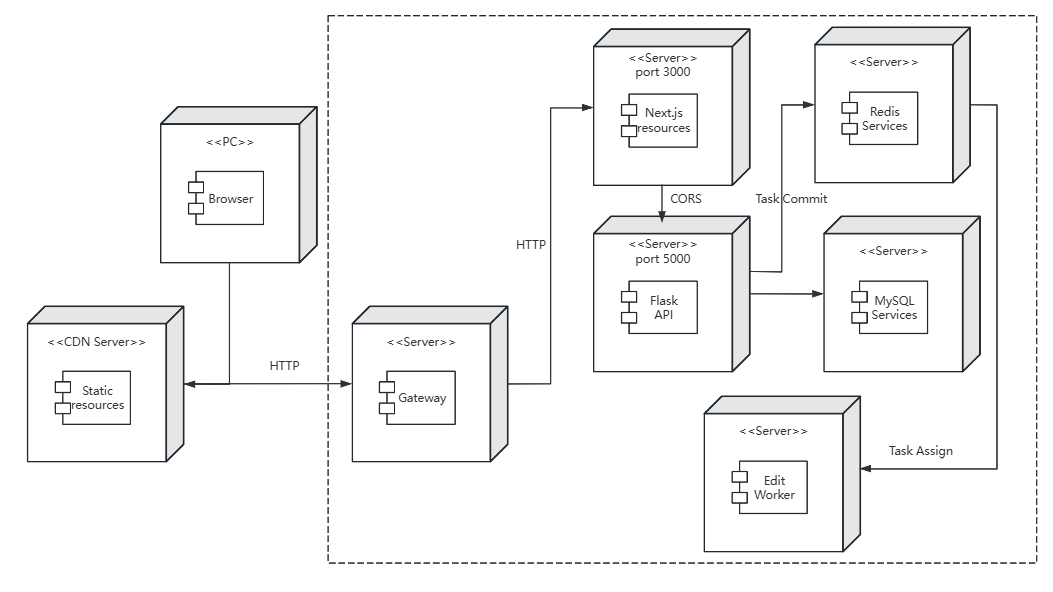
\includegraphics[width=0.7\textwidth]{source/img/system_deploy.png}
    \bicaption{系统物理视图}{Physical View}
    \label{fig:system-deploy}
\end{figure}

\subsection{数据库设计}

数据库作为后端存储的核心负责存储系统中的各种信息。我们将系统中的实体抽象为用户、请求任务、视频与图片文件,
使用数据实体关系(Entity Relationship, ER)图来描述这些实体及实体间的联系,我们设计的ER图如~\ref{fig:database-ER}所示。

\begin{figure}[ht]
    \centering
    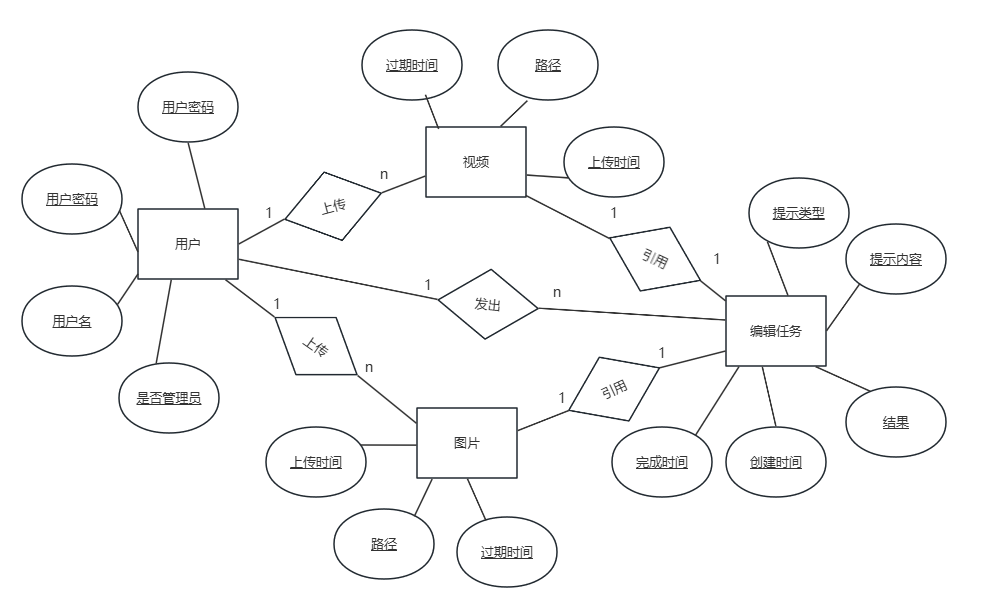
\includegraphics[width=0.6\textwidth]{source/img/database_ER.png}
    \bicaption{数据库ER图}{Database ER Diagram}
    \label{fig:database-ER}
\end{figure}

在实体关系图的基础上,我们进一步设计数据库的物理模型,如~\ref{fig:database-design}所示。本系统的数据库设计为用户表、任务表、视频表与图片表。

用户表除了存储~\ref{fig:database-ER}中列出的属性外,添加了用户id作为用户的唯一标识,设置为用户记录的主键。根据我们的
注册流程,用户表中的用户名、密码、邮箱、用户id均设置了非空约束,以保证用户信息的完整性。

任务表的设计在ER图中所示的属性基础上,直接添加了使用的文件信息与上传者信息,而不是全部采用外键关联的方式。我们采用这种设计出于两方面考虑:
一方面,为了防止后台文件积压,我们对已使用的文件也设置了过期时间,如果采用外键约束,文件过期后对应记录删除,任务表记录将不完整,这与我们期望获得完整任务信息
的需求不符;另一方面将任务所需全部信息都集中存储在一个表中,可以减少实际运行过程中的数据库查询次数,用空间换取了时间。与用户表的处理相同,
我们添加了任务id表项作为任务记录的唯一标识,并设置为主键。

在将任务所需信息全部集成在任务表中后,视频与图片两个文件表的功能就变得单一,仅作为文件过期删除功能的辅助表,存储文件的过期信息。但为了
保持数据库记录的一致性,我们仍然设置了外键引用,在两个表中分别引用了对应的任务id。

\begin{figure}[ht]
    \centering
    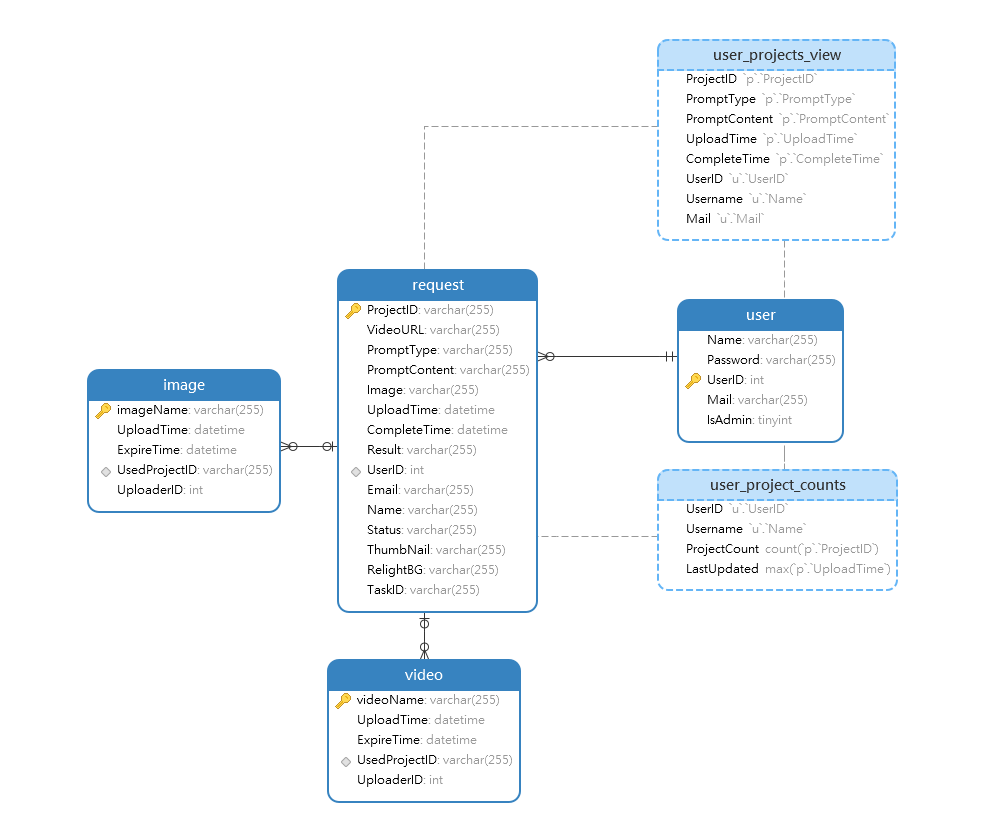
\includegraphics[width=0.6\textwidth]{source/img/database_design.png}
    \bicaption{数据库物理模型}{Database Physical Model}
    \label{fig:database-design}
\end{figure}
